\documentclass[a4paper,11pt]{article}
\usepackage{color}
\usepackage{graphicx}
\usepackage{subcaption}
\usepackage{wrapfig}
\usepackage[export]{adjustbox}
\usepackage{geometry}
\usepackage{setspace}
\usepackage{adjustbox}
\usepackage{amsmath}
\usepackage{textgreek}
\usepackage{url}
\usepackage{siunitx}
\usepackage{textcomp}
\usepackage[square,numbers]{natbib} %the big one
\doublespacing
\geometry{legalpaper, portrait, margin=2cm}
\begin{document}
\title{Open Science Hardware Setup for investigating the Stability of Organic Solar Cells - Interim Report}
\author{Samuel Mendis}
\date{\today}
\maketitle
\pagebreak
\section{Introduction}
Solar cells are becoming increasingly prevalent in the fight against climate change\cite[p.~XV]{RN45}, leading demand to increase worldwide. This project looks at helping design the next generation of solar cells to be manufactured out of organic material - rather than the current industry standard of Silicon. Currently, controlled lifetime testing of organic solar cells is difficult due to the multitude of failure mechanisms which arise due to chemical degradation via Oxygen and water\cite[p.~689]{RN38}. To help solve this problem, this project will design, manufacture and test a programmable lifetime solar testing container. A key aspect of this project is to be open hardware, this is to ensure that research groups around the world can use it if need be, which could potentially accelerate the development of organic solar cells. 

\section{Aims and Objectives}
The aim of the container is to simulate a lifetime (20 years) of real world degradation in a \emph{reasonable} timeframe. The ambiguity of reasonable is used as an ideal testing container should be able to test the solar cell in a short cycle test (15 minutes) or a long multiple cycle test (a period of days). To ensure accurate testing of the cells, the container needs to be airtight. This is to prevent any atmospheric Oxygen and water vapour getting into the container and causing unwanted degradation of the cell. Furthermore, the container is going to have gas inlets and outlets so that the conditions that the solar cell is tested under can be varied. This will be in conjunction with a temperature controller capable of varying the temperature of the solar cell up to 120\textdegree C. These objectives were guided by the paper \emph{Consensus stability testing protocols for organic photovoltaic materials and devices} \cite[p.~1255-1261]{RN47} which cites multiple different testing criteria for an organic solar cell. Further criteria which would enhance the scope of the project is a graphical user interface (GUI) developed to control the conditions within the testing container. These are all achievable aims within the timeframe allowed, which can be clearly seen on the Gantt chart attached. 

\section{Progress}
At this stage in the year, the testing container is past the design stage and is onto manufacturing. A full design has been completed using the open source software OpenSCAD. Using inspiration from X an AMFD researcher (who had developed a similar type of device, without the functionality) a CAD model of the testing container was built and is shown in Figure \ref{fig:model} below. \\
\begin{figure}[h]
\begin{subfigure}{0.5\textwidth}
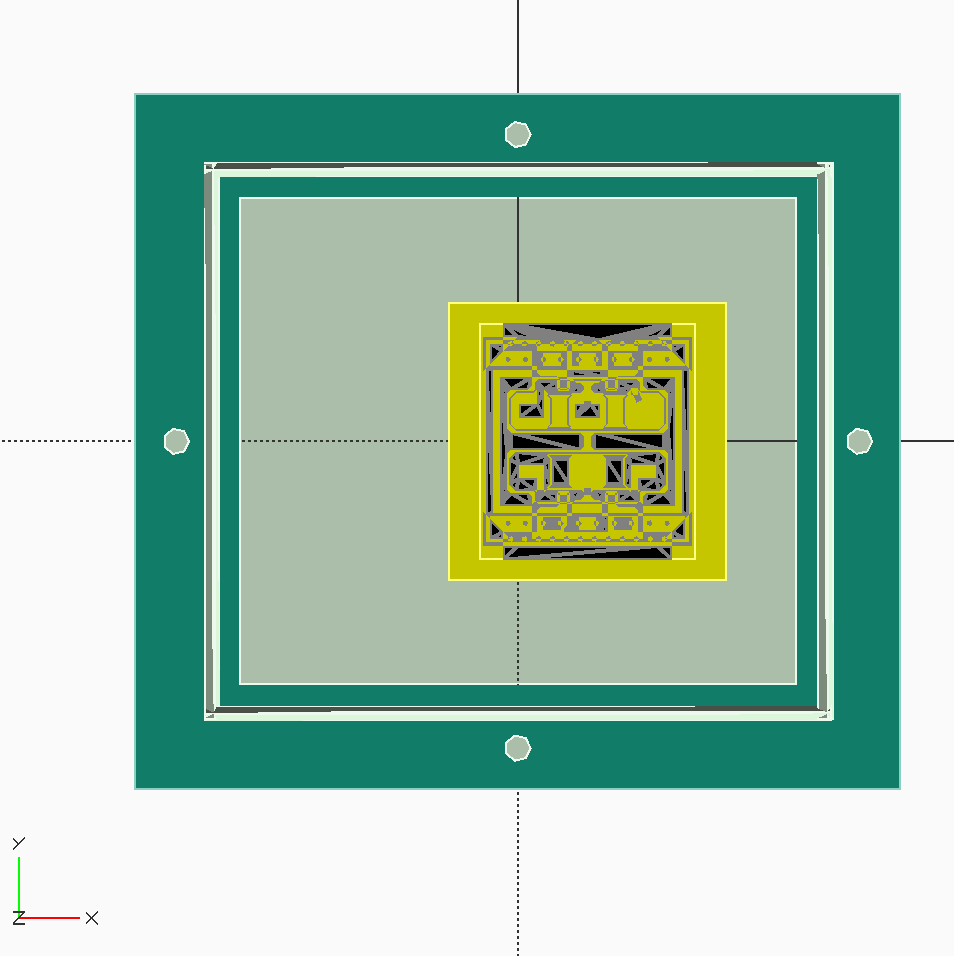
\includegraphics[width=0.9\linewidth]{fig1a}
\caption{Plan View of Model}
\label{fig:subim1}
\end{subfigure} \begin{subfigure}{0.5\textwidth}
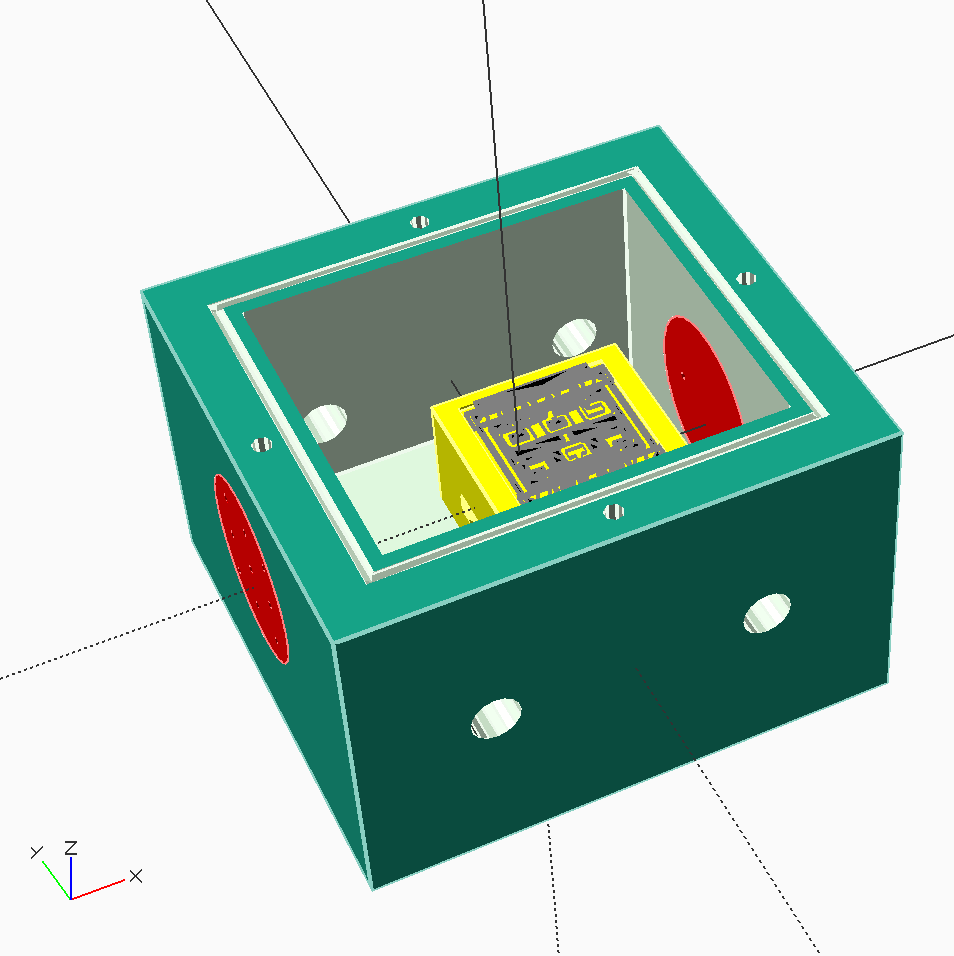
\includegraphics[width=0.9\linewidth]{fig1b}
\caption{Isometric View of Model}
\label{fig:subim2}
\end{subfigure}
\caption{Showing plan and isometric view of the full OpenSCAD model\label{fig:model}}
\label{fig:image2}
\end{figure}
\noindent The design needed to fit the substrate (black), any electronic devices and gas inlet ports. The substrate used carries 8 solar cells with dimensions of 30 mm * 30 mm and a thickness of 1 mm, this can be seen in Figure \ref{fig:substrate} which is a model of the substrate used provided by Dr. Grey Christophoro . To cary the substrate in the container a substrate holder was designed to fit within the outer shell of the container allowing a more modular design for the container. This modular design is desirable as it allows the ability to modify the cells which are being tested without the redesign of the entire container, just a the parts needed, thereby saving those who may need to use it in the future valuable time and money. 
\\
\\
\begin{wrapfigure}{b}{0.35\textwidth} 
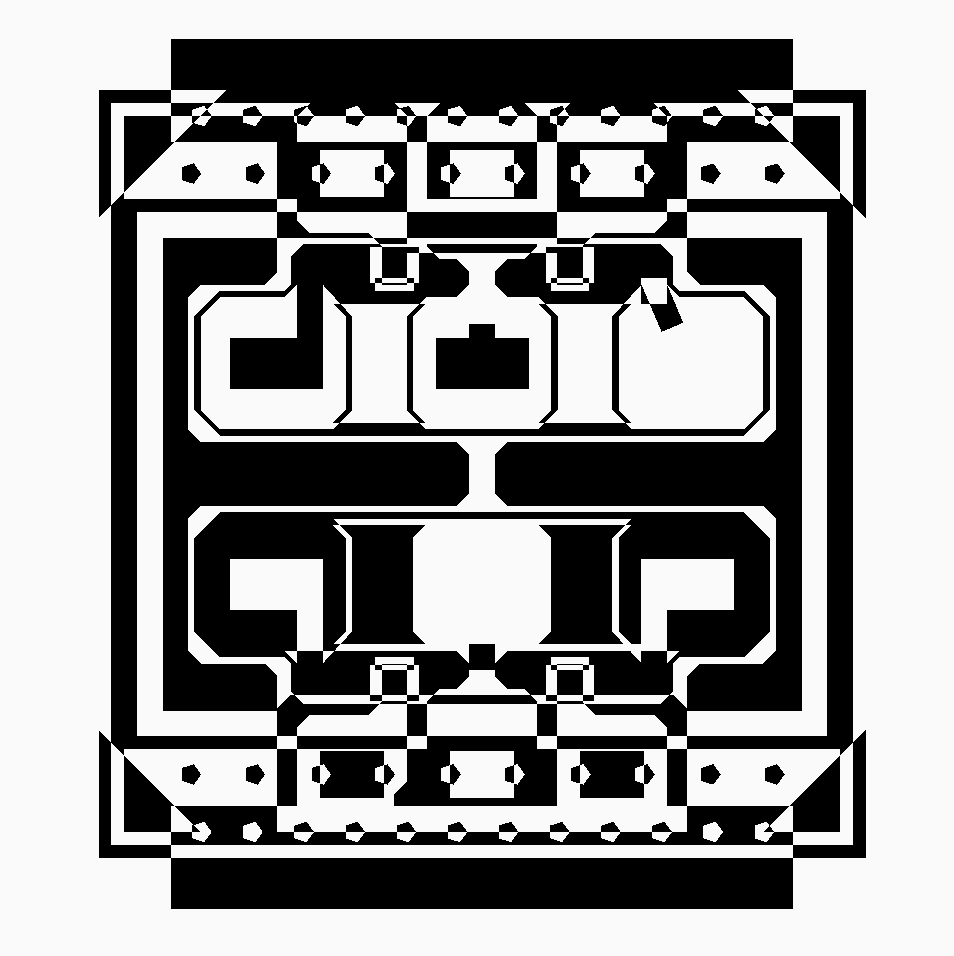
\includegraphics[width=\linewidth]{fig2}
\caption{Model of Substrate provided by Dr. Grey Christophoro\label{fig:substrate}}
\end{wrapfigure}\noindent Following the design of the model, prototypes were 3D printed in Acrylonitrile Butadiene Styrene (ABS) using the engineering faculties 3D printing facilities to ensure all the parts were the correct sizes and fitted with the purchased components.  These included a set of O-rings to seal the outer shell to the quartz window, push-fit valves for an easy connection between the gas pipes and the container and a pressure relief valve to ensure the safety of the pressurised box. These components were bought in, rather than manufactured, as these specific components are widely available worldwide thereby making it far more cost effective to buy from a supplier who creates the components in bulk, rather than creating bespoke parts in-house. 
\\
\\
The next important decision was what materials the container would be made from. The main objectives were to be corrosion resistant, lightweight and strong which is why Aluminium alloys were chosen as a good starting point for the outer shell. Research was undertaken to narrow the list down to four different alloys listed in the table below.
\begin{table}[h]
\begin{adjustbox}{width=1\textwidth}
\small
\begin{tabular}{|c|c|c|c|c|}
\hline
 Alloy&Density/kgm\textsuperscript{-3}&Corrosion resistance&Workability&Cost to make outer shell\\
 \hline
 AL-1100&2710&Excellent&Excellent&£100\\
 \hline
 AL-3003&2730&Excellent&Very Good&£100\\
 \hline
  AL-5052&2680&Excellent - Particularly marine environments&Good&£100\\
 \hline
 \end{tabular}
\end{adjustbox}
 \caption{Showing the parts purchased to date, their function and cost} 
\end{table}
 \noindent As can be seen these alloys are similar in most aspects leaving the only differentiator to be cost. After contacting the University workshops, they recommended the use of x alloy for the lowest cost. Once the material for the outer shell was chosen, the next objective was to decide on which material would be used for the window. After consultation with the AFMD research group it was clear that the material used for the window had to allow UV wavelengths through narrowing the choice down to quartz. Quartz is a good transmitter of UV light allowing the solar cell to experience solar conditions which would be experienced on earth - following the AM1.5 graph shown in the appendix. The quartz transmission graph is also shown within the appendix.

\section{What next?}
Once in receipt of the outer shell and quartz window the next steps would be to pressure test the vessel. This can be done in a variety of different ways, placing the vessel underwater, pressurising the vessel with a dyed air and seeing if there is any leakage. Once confirmed that the vessel is sealed, it will be possible to start working on the control electronics for the systems. This involves calibrating the heating element and temperature sensors as well as creating a controller to modify the environmental conditions. These tasks will require lots of time in the lab to ensure reliability of the container, which is why I have identified it as a potential bottleneck and have planned accordingly. As can be seen from the Gantt chart shown as appendix 1, this section is forecast to take many weeks which as there may be problems when using these components due to a lack of experience. Once the calibration is complete the container will undergo many tests to see if the solar cell reacts as predicted (failing under certain conditions, surviving under inert environments). If this proceeds as predicted in the Gantt chart the project should be finished by the end of Hillary term, giving 6 weeks contingency if any unforeseen problems crop up. 

\bibliographystyle{ieeetr} %also the big one 
\bibliography{untitled}


\end{document}